% Figure: the signaling geometry. Referenced from §9's lead. Pure TikZ, design after the
% hub's memory_halfline.py (the boundary-fed half-line), adapted: the axes are (t, x),
% the signal enters ONLY at the boundary x = 0, the field u(t,x) is carried by the
% time evolution ∂_t u = A u along the memory line, and the two transforms act in the
% two different variables.

\begin{figure}[t]
\centering
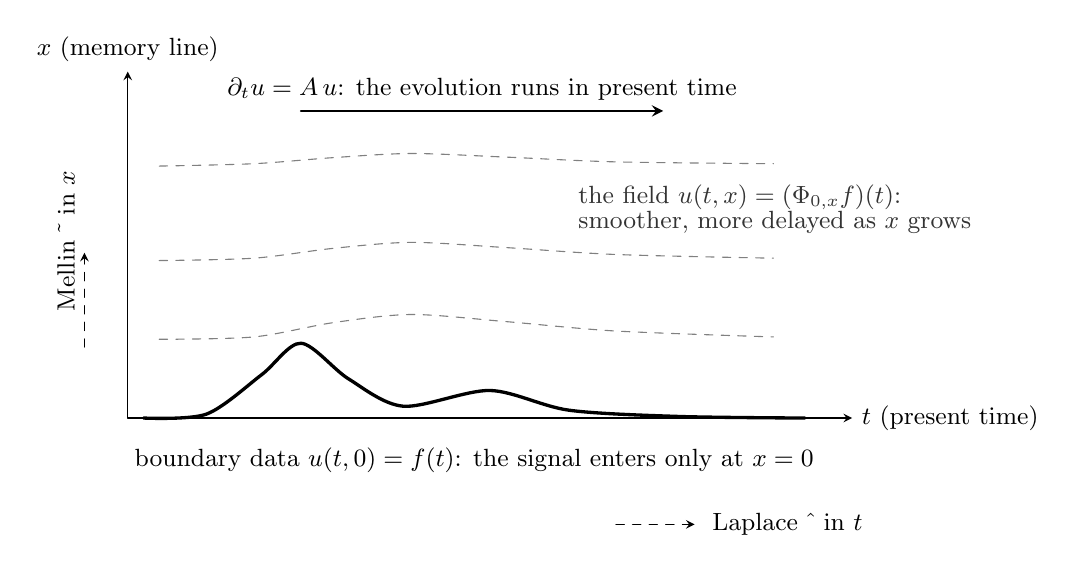
\begin{tikzpicture}[every node/.style={font=\small}, line cap=round, >=stealth]

% axes
\draw[->] (0,0) -- (9.2,0) node[right] {$t$ (present time)};
\draw[->] (0,0) -- (0,4.4) node[above] {$x$ (memory line)};

% boundary data: a transient signal along the t-axis
\draw[very thick]
  plot[smooth] coordinates {(0.2,0) (1.0,0.05) (1.7,0.55) (2.2,0.95) (2.8,0.5) (3.5,0.15) (4.6,0.35) (5.6,0.1) (7.0,0.02) (8.6,0)};
\node[anchor=north] at (4.4,-0.25) {boundary data $u(t,0) = f(t)$: the signal enters only at $x = 0$};

% the field in the interior: dashed level profiles
\foreach \x/\o in {1.0/0.75, 2.0/0.55, 3.2/0.38} {
  \draw[gray,dashed]
    plot[smooth] coordinates {(0.4,\x) (1.6,\x+0.03) (2.6,\x+0.28*\o) (3.6,\x+0.42*\o) (4.8,\x+0.30*\o) (6.2,\x+0.14*\o) (8.2,\x+0.03)};
}
\node[gray!40!black,anchor=west] at (5.6,2.80) {the field $u(t,x) = (\Phi_{0,x}f)(t)$:};
\node[gray!40!black,anchor=west] at (5.6,2.48) {smoother, more delayed as $x$ grows};

% the evolution arrow: in time, at fixed depth
\draw[->,thick] (2.2,3.9) -- node[above] {$\partial_t u = A\,u$: the evolution runs in present time} (6.8,3.9);

% the two transforms
\draw[->,dashed] (-0.55,0.9) -- (-0.55,2.1);
\node[rotate=90,anchor=south] at (-0.55,2.25) {Mellin $\tilde{\ }$ in $x$};
\draw[->,dashed] (6.2,-1.35) -- (7.2,-1.35);
\node[anchor=west] at (7.3,-1.35) {Laplace $\hat{\ }$ in $t$};

\end{tikzpicture}
\caption{The signaling geometry. The signal is never stored: it enters the device only as
boundary data at zero scale, and what the observer carries is the field $u(t,x)$ over the
memory half-line --- at each fixed $x$ a record of the signal at that scale, smoother and more
delayed as $x$ grows. Theorem~\ref{thm:signaling-form} inverts the scale evolution into an
evolution \emph{in present time}: $\partial_t u = A u$, with $A$ acting along the memory line
only. The section works with two transforms in two different variables: the Laplace transform
$\hat{\ }$ in $t$, in which the field at fixed $s$ is a dilate $\hat f(s)H(sx)$ of one
profile, and the Mellin transform $\tilde{\ }$ in $x$, in which $A$ is diagonal with symbol
$B$.}
\label{fig:signaling}
\end{figure}
